\documentclass[14pt]{extbook}
\usepackage{multicol, enumerate, enumitem, hyperref, color, soul, setspace, parskip, fancyhdr} %General Packages
\usepackage{amssymb, amsthm, amsmath, latexsym, units, mathtools} %Math Packages
\everymath{\displaystyle} %All math in Display Style
% Packages with additional options
\usepackage[headsep=0.5cm,headheight=12pt, left=1 in,right= 1 in,top= 1 in,bottom= 1 in]{geometry}
\usepackage[usenames,dvipsnames]{xcolor}
\usepackage{dashrule}  % Package to use the command below to create lines between items
\newcommand{\litem}[1]{\item#1\hspace*{-1cm}\rule{\textwidth}{0.4pt}}
\pagestyle{fancy}
\lhead{Progress Quiz 8}
\chead{}
\rhead{Version B}
\lfoot{5493-4176}
\cfoot{}
\rfoot{Summer C 2021}
\begin{document}

\begin{enumerate}
\litem{
First, find the equation of the line containing the two points below. Then, write the equation in the form $ y=mx+b $ and choose the intervals that contain $m$ and $b$.\[ (6, -7) \text{ and } (11, 6) \]\begin{enumerate}[label=\Alph*.]
\item \( m \in [-8.6, -1.6] \hspace*{3mm} b \in [33.6, 36.6] \)
\item \( m \in [-0.4, 6.6] \hspace*{3mm} b \in [18.6, 28.6] \)
\item \( m \in [-0.4, 6.6] \hspace*{3mm} b \in [-22.6, -20.6] \)
\item \( m \in [-0.4, 6.6] \hspace*{3mm} b \in [-11, -3] \)
\item \( m \in [-0.4, 6.6] \hspace*{3mm} b \in [-15, -11] \)

\end{enumerate} }
\litem{
Solve the equation below. Then, choose the interval that contains the solution.\[ -12(-14x + 17) = -4(-19x + 2) \]\begin{enumerate}[label=\Alph*.]
\item \( x \in [1.94, 2.27] \)
\item \( x \in [2.17, 2.43] \)
\item \( x \in [-2.67, -2.23] \)
\item \( x \in [0.78, 1.12] \)
\item \( \text{There are no real solutions.} \)

\end{enumerate} }
\litem{
Write the equation of the line in the graph below in Standard Form $Ax+By=C$. Then, choose the intervals that contain $A, B, \text{ and } C$.
\begin{center}
    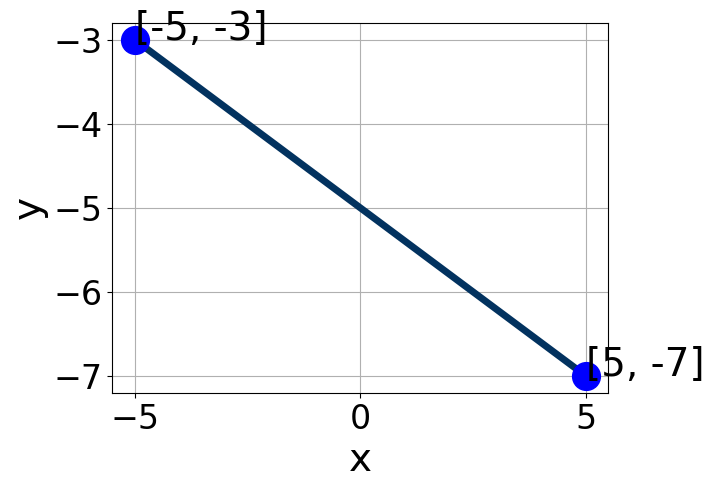
\includegraphics[width=0.5\textwidth]{../Figures/linearGraphToStandardB.png}
\end{center}
\begin{enumerate}[label=\Alph*.]
\item \( A \in [0.1, 1.5], \hspace{3mm} B \in [0.6, 1.8], \text{ and } \hspace{3mm} C \in [-10, -1] \)
\item \( A \in [0.1, 1.5], \hspace{3mm} B \in [-1.4, 0.1], \text{ and } \hspace{3mm} C \in [3, 7] \)
\item \( A \in [1.1, 4.4], \hspace{3mm} B \in [3.4, 7.4], \text{ and } \hspace{3mm} C \in [-26, -24] \)
\item \( A \in [-2.2, -0.9], \hspace{3mm} B \in [-6.1, -4.8], \text{ and } \hspace{3mm} C \in [20, 32] \)
\item \( A \in [1.1, 4.4], \hspace{3mm} B \in [-6.1, -4.8], \text{ and } \hspace{3mm} C \in [20, 32] \)

\end{enumerate} }
\litem{
Find the equation of the line described below. Write the linear equation in the form $ y=mx+b $ and choose the intervals that contain $m$ and $b$.\[ \text{Parallel to } 6 x - 7 y = 13 \text{ and passing through the point } (2, -5). \]\begin{enumerate}[label=\Alph*.]
\item \( m \in [1.13, 2.36] \hspace*{3mm} b \in [-6.84, -4.95] \)
\item \( m \in [-0.01, 1.02] \hspace*{3mm} b \in [-6.84, -4.95] \)
\item \( m \in [-0.01, 1.02] \hspace*{3mm} b \in [6.69, 7.89] \)
\item \( m \in [-0.01, 1.02] \hspace*{3mm} b \in [-7.39, -6.76] \)
\item \( m \in [-1.34, -0.72] \hspace*{3mm} b \in [-3.91, -2.08] \)

\end{enumerate} }
\litem{
Solve the linear equation below. Then, choose the interval that contains the solution.\[ \frac{4x -5}{4} - \frac{5x + 5}{3} = \frac{-8x -9}{8} \]\begin{enumerate}[label=\Alph*.]
\item \( x \in [-0.7, 1.1] \)
\item \( x \in [-4.8, -3] \)
\item \( x \in [5.2, 7.6] \)
\item \( x \in [2.8, 4.1] \)
\item \( \text{There are no real solutions.} \)

\end{enumerate} }
\litem{
Find the equation of the line described below. Write the linear equation in the form $ y=mx+b $ and choose the intervals that contain $m$ and $b$.\[ \text{Parallel to } 6 x + 5 y = 7 \text{ and passing through the point } (-3, -10). \]\begin{enumerate}[label=\Alph*.]
\item \( m \in [-1.12, -0.75] \hspace*{3mm} b \in [-14, -12.98] \)
\item \( m \in [-2.5, -0.92] \hspace*{3mm} b \in [13.21, 13.82] \)
\item \( m \in [0.75, 1.71] \hspace*{3mm} b \in [-6.99, -6.29] \)
\item \( m \in [-2.5, -0.92] \hspace*{3mm} b \in [-14, -12.98] \)
\item \( m \in [-2.5, -0.92] \hspace*{3mm} b \in [-7.27, -6.62] \)

\end{enumerate} }
\litem{
Solve the equation below. Then, choose the interval that contains the solution.\[ -18(19x -12) = -13(-15x -14) \]\begin{enumerate}[label=\Alph*.]
\item \( x \in [-0.8, -0.54] \)
\item \( x \in [0.05, 0.16] \)
\item \( x \in [2.66, 2.9] \)
\item \( x \in [0.58, 1.12] \)
\item \( \text{There are no real solutions.} \)

\end{enumerate} }
\litem{
First, find the equation of the line containing the two points below. Then, write the equation in the form $ y=mx+b $ and choose the intervals that contain $m$ and $b$.\[ (9, 5) \text{ and } (10, -5) \]\begin{enumerate}[label=\Alph*.]
\item \( m \in [-12, -6] \hspace*{3mm} b \in [-4, 0] \)
\item \( m \in [-12, -6] \hspace*{3mm} b \in [-95, -91] \)
\item \( m \in [-12, -6] \hspace*{3mm} b \in [93, 103] \)
\item \( m \in [-12, -6] \hspace*{3mm} b \in [-16, -13] \)
\item \( m \in [8, 15] \hspace*{3mm} b \in [-105, -102] \)

\end{enumerate} }
\litem{
Write the equation of the line in the graph below in Standard Form $Ax+By=C$. Then, choose the intervals that contain $A, B, \text{ and } C$.
\begin{center}
    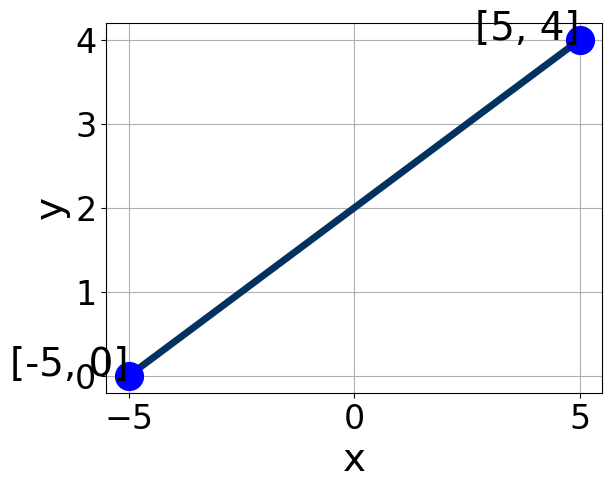
\includegraphics[width=0.5\textwidth]{../Figures/linearGraphToStandardCopyB.png}
\end{center}
\begin{enumerate}[label=\Alph*.]
\item \( A \in [-6.4, -1.5], \hspace{3mm} B \in [1.2, 6.5], \text{ and } \hspace{3mm} C \in [4, 12] \)
\item \( A \in [0.8, 5.6], \hspace{3mm} B \in [-5.3, -3.1], \text{ and } \hspace{3mm} C \in [-15, -5] \)
\item \( A \in [-1.3, -0.3], \hspace{3mm} B \in [-1.7, -0.3], \text{ and } \hspace{3mm} C \in [-8, 1] \)
\item \( A \in [0.8, 5.6], \hspace{3mm} B \in [1.2, 6.5], \text{ and } \hspace{3mm} C \in [4, 12] \)
\item \( A \in [-1.3, -0.3], \hspace{3mm} B \in [0.7, 3.9], \text{ and } \hspace{3mm} C \in [1, 5] \)

\end{enumerate} }
\litem{
Solve the linear equation below. Then, choose the interval that contains the solution.\[ \frac{8x -7}{5} - \frac{5x -3}{4} = \frac{7x + 6}{7} \]\begin{enumerate}[label=\Alph*.]
\item \( x \in [-4.32, -1.32] \)
\item \( x \in [-5.63, -3.63] \)
\item \( x \in [-0.38, 2.62] \)
\item \( x \in [-16.38, -14.38] \)
\item \( \text{There are no real solutions.} \)

\end{enumerate} }
\end{enumerate}

\end{document}